\documentclass{mpaper}

\begin{document}

\title{Measuring Software Ticket Quality using Quantitative Data Analysis}
\author{Andrei-Mihai Nicolae}
\matricnum{21473292}

\maketitle

\begin{abstract}
Issue trackins systems have become the defacto standard for tracking work items in 
software projects - they guide engineers towards better planning and 
managing their progress throughout complex projects. However, there
are few studies that investigate what makes for a high quality,
valuable ticket. This can lead to multiple issues in a company, such as 
increased communication friction between developers and end users filing bug
reports, as well as increased overall costs due to waste of development effort. 
In this research paper, we present our findings after 
investigating a large number of variables surrounding software tickets, 
Our results show that the presence and type of attachments,
comments complexity, summary and description complexity, presence of stack traces, presence
of steps to reproduce, grammar correctness scores, as well as sentiment can significantly influence 
the quality of the ticket. We supply one of the largest dataset statistically 
analysed in this particular field, as well as state-of-the-art sentiment and grammar correctness analyses.
\end{abstract}

\section{Introduction}\label{intro}

In the past decade software projects have inherently become more complex and require increasing number of developers in
the team. Studies such as the one conducted by Herbsleb \cite{herbsleb2007global} show how software engineering teams have 
transitioned from small, collocated to globally distributed teams. One reason elicited in the paper is the increasing 
popularity of communication tools, such as Slack or Google Hangouts. Due to this, developers have created issue tracking 
systems as means of planning, managing and tracking work products in the form of \emph{software tickets} or \emph{issues}.

There are multiple platforms for providing such issue tracking systems, among which
the most popular are Jira and Bugzilla. For both platforms,
the tickets are split into two main categories: feature requests (i.e. feature to be 
implemented into the system) and bug reports (i.e. issue encountered by an end user or
discovered by a developer in the codebase). Regardless of the type of ticket, they possess
various information that can be filled in by the reporter (i.e. person who created the ticket; 
can be both an end user or a developer in the team), providing the developers
a detailed view of what is requested or what went wrong.

Even though tickets provide such comprehensive data regarding a specific task, studies have shown 
that fixing bugs is one of the most common and time consuming tasks performed by developers \cite{latoza2006maintaining}. One of
the reasons for this is the communication friction between developers and end users \cite{Korkala2014WasteIdentification}
as developers might need clarification regarding what information the users have provided (e.g. cannot reproduce the bug, 
screenshot is unclear). Another main reason for this waste of effort on solving tickets, according to 
Just et. al \cite{just2008towards} and Zimmermann et. al \cite{zimmermann2009improving}, is the generally poor design of issue 
tracking systems. This can lead to various issues, including increased costs for the company, wasted development effort, 
decreased customer satisfaction and overall poor performance.

Therefore, there is a need in the community to find the answer to what makes for a high quality, valuable software ticket 
that would improve the overall performance of the development team and, inherently, the company. As there are many 
fields in a ticket, there are numerous unanswered questions, such as whether stack traces have an influence on the quality
of a ticket? 

In this research paper, we present and discuss our findings after running a quantitative data analysis 
on over 3200,000 tickets taken from more than 15 open source projects. We have implemented a Go application 
with multiple commands (i.e. store, analyze, plot, statistics) that can automatically fetch any number of tickets 
from a Jira instance, analyze them, generate plots and run statistical tests. 

During the analysis part, we investigate several variables in correlation with \emph{Time-To-Close}, 
which we define as the \emph{metric of quality}. \emph{Time-To-Close} represents the period of time between the creation 
and the closing of a ticket; more specifically, the creation of the ticket is marked when the status of the ticket is set to 
\emph{Open} and the closing of a ticket is considered when the ticket status is set to \emph{Closed} (or some similar status, 
such as \emph{Fixed}, \emph{Resolved}). \emph{Time-To-Close} is our dependent variable, and as independent variables 
(i.e. variables controlled in order to test the effects on the dependent variable) we have set a number of ticket fields. 

In order to provide answers to what factors influence quality in a software ticket, we answer the following seven research 
questions in this paper (Section \ref{correlations}):
\begin{itemize}
  \item does the presence of attachments and their type (e.g. code snippet, screenshot) influence the \emph{Time-To-Close} for 
  a ticket?
  \item does the presence of stack traces improve the ticket quality?
  \item does the presence of steps to reproduce reduce the \emph{Time-To-Close}?
  \item is there a relationship between the number of words in comments and \emph{Time-To-Close}?
  \item does the total number of words in summary and description have an impact on \emph{Time-To-Close}?
  \item does the number of grammar errors in summary, description and comments have an effect on the quality of a ticket?
  \item does a positive or negative ticket influence its \emph{Time-To-Close}?
\end{itemize}

This study brings several contributions to the research community:
\begin{itemize}
  \item an innovative tool was built for the purpose of this project, providing efficient data collection and analysis of
  tickets;
  \item it is one of the few studies in the field that performs a quantitative analysis rather than a qualitative one;
  \item it is one of the very few research projects that investigates such a large number of tickets (over 300,000)
  extracted from 38 different projects;
  \item it is, to our knowledge, the first study to conduct sentiment and grammar correctness analyses on software tickets.
\end{itemize}

The rest of the paper is structured as follows. In Section \ref{related_work} we iterate over state-of-the art studies in 
the field and then continue with Section \ref{building} where we discuss how the ticket data set was collected and 
analysed. We continue with describing the data set (Section \ref{characterising}) where we provide insights into various 
aspects of the data (e.g. size of database, number of tickets with attachments) and then discuss correlations between 
the variables (Section \ref{correlations}). Finally, we provide future research directions in Section \ref{future_work} 
and present our conclusions in Section \ref{conclusions}.

\section{Related Work}\label{related_work}

In this section we will present what are the state-of-the art studies in the issue/ticket quality 
field. More specifically, we will look at research papers that investigated what makes for a valuable ticket, 
how can one extract structured/unstructured data from tickets (e.g. stack traces), ticket duplication and its 
positive and negative outcomes, quality of modern issue tracking systems as well as automating the process 
of summarizing tickets or the optimal assignee. 

The study of Bettenburg et. al \cite{bettenburg2008makes} showed what 
makes for a valuable bug report through qualitative analysis. 
After conducting interviews with over 450 developers, Bettenburg et. al concluded that one of the main factors
behind a quality ticket is grammar correctness in summary and description. Another
aspect which was flagged as helpful by the interviewees was the presence of stack 
traces and steps to reproduce in tickets. A further contribution brought by the
authors to the community is the creation of a tool called Cuezilla which is able 
to automatically predict the quality of a bug report with an accuracy of around 40\%.

Another research paper that strenghtens the argument that readability is a quality 
factor in software tickets is the one presented by Hooimeijer et. al \cite{hooimeijer2007modeling}.
They conducted their analysis on over 25,000 bug reports from the Mozilla project, 
investigating readability, daily load, submitter reputation, the whole changelog histories 
and severity. They conclude that not only readability in the textual fields of a ticket
influence the \emph{Time-To-Close}, but also that the presence of attachments and 
the number of comments have a clear effect on the duration of triaging. On the 
other hand, the patch count and other similar fields did not provide significant 
value to the quality of tickets.

However, there are other types on information typically included in software tickets 
which might prove beneficial for developers and subsequently improve the ticket quality.
One such type is stack traces and Schroter et. al \cite{schroter2010stack} analyse how 
quickly tickets are closed when they either have stack traces included in their fields 
(e.g. description) or not. They collected their data from the Eclipse project using 
the InfoZilla tool proposed by Bettenburg et. al \cite{bettenburg2008extracting}.
Then, they linked the stack traces to changes in source code by mining the Eclipse version 
controlled repository. The results showed that 
around 60\% of the bugs that contained stack traces in their reports were fixed
in one of the methods in the frame. Moreover, more than 40\% of the tickets having stack traces
got fixed in the first stack frame.

Software tickets can have duplicates, usually meaning that the most important fields, such 
as summary or description, describe the same feature request or bug report. Even though 
one might believe that they cannot bring any value to a software project, the work of 
Bettenburg et. al \cite{bettenburg2008duplicate} shows the contrary.
The authors collected large amounts of data from the Eclipse open source project and ran
various kind of textual and statistical analysis on the data to find answers.
After the results were computed, they concluded that usually bug duplicates contain 
information that is not present in the master report (i.e. the original report that was 
filed). Also, developers also specified that they have often found value in these 
duplicate bug reports and that they can even aid automated triaging techniques. 

%TODO: ADD HERE PROPER PAPER
However, the study conducted by Cavalcanti et. al \cite{cavalcanti2013bug} shows completely 
different results. The authors investigated around 280,000 tickets from multiple open and 
closed source repositories and found that having bug duplicates
97,000 tickets from the Mozilla repository in order to infer the quality of merging duplicate
bug reports. Their results are statistically significant and they show that merging bug report 
duplicates improved the overall quality of the project (i.e. ) 

Bettenburg et. al \cite{bettenburg2012using} present in their work an application
called infoZilla. This tool can
parse bug reports and correctly extract stack traces, patches and source code. 
When evaluated on over 150,000 bug reports, it proved to have a very high rate of over 97\% accuracy.
We applied some of the techniques shown in the study and successfully managed to 
retrieve stack traces as well with a great accuracy.

The first information to be filled in by end users or developers on any issue tracking system
is the summary field, which holds a small description, usually between 5 and 30 words, of 
the request or bug being reported. In the study conducted by Rastkar et. al \cite{rastkar2010summarizing}, 
the authors investigated whether tickets could be summarized automatically and efficiently. What 
that implies is that developers would not be required to look at complete tickets comprised 
of a large number of fields, but rather at a simple summary of a couple of lines 
encapsulating the whole information. The authors selected the Mozilla, Eclipse, Gnome and KDE 
open source projects and then they asked volunteering university students to annotate 
the tickets in the issue tracking systems. More specifically, they had to write a summary 
of maximum 250 words using both technical and non-technical terms, depending on their expertise. 
Then, the study presents Machine Learning algorithms employed to parse these summaries and 
learn how to efficiently create automated summaries for new bug reports. Afterwards, they asked 
software developers to rate these auto-generated summaries against the original ones and 
the conclusion was that existing conversation-based extractive summary generators used 
for software tickets produce the best results.

The work of Just et. al \cite{just2008towards} examines a rather different aspect
of quality in tickets - they are investigating the quality of the underlying issue 
tracking systems instead. 
The authors ran a survey on 175 developers from Eclipse, Apache and Mozilla
Then, they applied a card sort in order to organize the comments into hierarchies to 
identify common patterns. Their findings can be summarized in the following top seven
suggestions:
  \begin{itemize}
    \item create differentiation between bug report difficulty levels between 
    novices and experiences reporters;
    \item encourage users to input as much information as possible;
    \item add ability to merge tickets when needed;
    \item recognise and reward valuable bug reporters;
    \item integrate reputation into user profiles to mark experienced reporters;
    \item to be able to easily and expressively search through tickets.
  \end{itemize}

Having discussed about various factors that can influence the quality in software tickets, 
we also need to take into account how can we apply this knowledge to solving the issue of 
poor design in issue tracking systems and how the ticket creation process could be improved. 
The study conducted by Lamkanfi et. al \cite{lamkanfi2010predicting} looks at this aspect and
shows how issue tracking systems could be extended in order to automatically generate the severity 
of a ticket (e.g. assign story points to a Jira issue). The authors conducted their research on the Mozilla,
GNOME and Eclipse and projects and split their approach into four steps: extract and organize tickets, 
pre-process tickets (i.e. tokenization, stop word removal and stemming), train the classifier on two datasets 
of tickets - 70\% training and 30\% evaluation and apply the trained classifier on the evaluation set.
The conclusions they drew from running the evaluation process were rather 
interesting:
  \begin{itemize}
    \item terms such as segfault, deadlock, crash, hand or memory typically indicate
      a severe bug;
    \item when analyzing the textual description they found that using simple
      one line summaries resulted in less false positives and increased precision
      levels;
    \item the classifier needs a large number of tickets in order to predict correctly;
    \item depending on how well a software project is modularised, one can 
      use a predictor per module rather than a universal one.
  \end{itemize}

Another overall aspect of software tickets and issue tracking systems that could be improved through 
determining the quality factors for tickets is automatically assigning a bug report or a feature request 
to the most suitable developer (or team of developers). Anvik et. al \cite{anvik2011reducing}
propose a Machine Learning technique that could automatically assign a bug report to the developer 
with the most expertise in that specific area. Firstly, the algorithm takes as input various types of information from 
tickets: textual description and summary, operating system used when the bug occurred, developer 
who owns the source code, which developers have lighter workloads at that point in time etc. After the 
tool was evaluated, the authors concluded that it can be used in production as it provides a high 
rate of accuracy when assigning the developers, but it needs more data so that the model is trained 
properly.

\begin{figure*}
\begin{center}
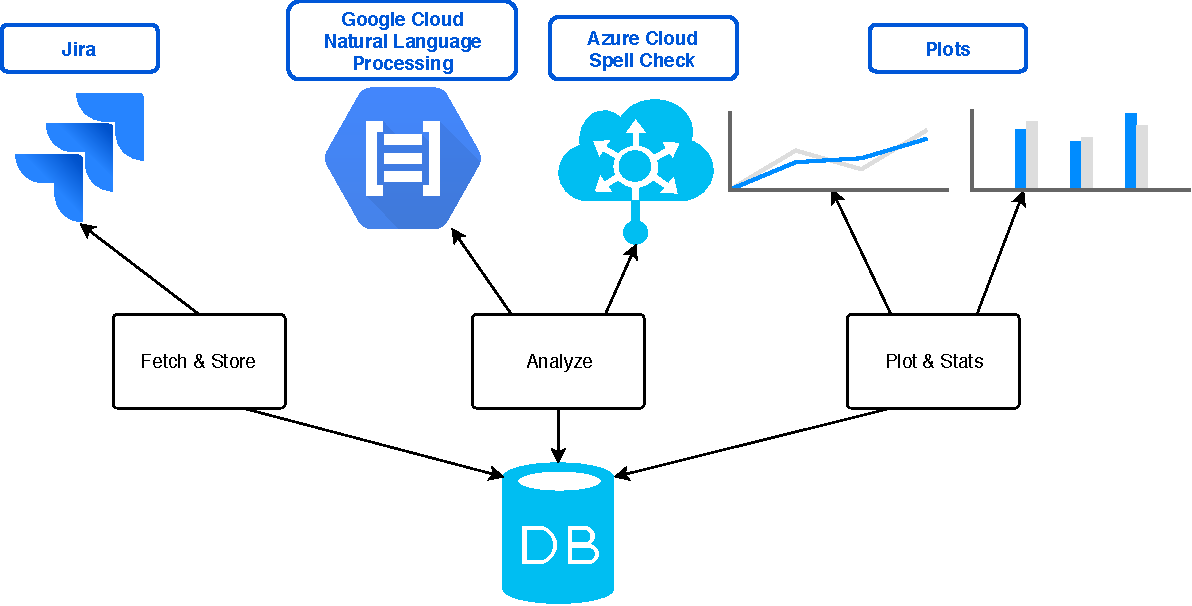
\includegraphics[width=\textwidth]{images/flow.pdf}
\end{center}
\caption{\label{fig-eg}Application flow of the Go tool.}
\end{figure*}

\section{Building the Data Set}\label{building}
The first step towards building the data set was to create a tool that was able to execute all the commands that we required:
fetching the tickets from any Jira instance, storing them into some form of database, analyze the variables of interest, 
automatically plot the correlations between them and run statistical analysis on the data. After careful consideration, 
we decided that Go was the best way to go for various reasons:
  \begin{itemize}
    \item it is designed with simplicity in mind, thus making it easy for others who might join the project to read 
    and understand the codebase; this would prove useful for us as developing the tool further is on our list of future 
    work items;
    \item it is a compiled, statically typed language that produces cross-platform executables when building the application;
    this is helpful for our research as we can use any machine or cluster of computers regardless of the operating system 
    running on them and collect even larger number of tickets than what we have collected so far;
    \item is is designed with concurrency in mind, thus it helps reduce times of execution and computing power considerably;
    in our case, why it helps us is by allowing access to goroutines, very lightweight threads that can scale even up to 
    millions; we use this powerful concept while fetching tickets from Jira or storing in the database - at one point, we had 
    more than 30,000 goroutines running at the same time.
  \end{itemize}

Throughout the entire application, we tried to apply the UNIX philosophy of creating small applications that do one thing, but 
do it well. Therefore, we implemented clean and simple packages where we tried to use the standard library as much as possible
so that potential contributors coming to the project would find it easy to start working directly on the code. Also, we designed 
the tool with extensibility in mind, so that other database providers (e.g. CockroachDB) or issue tracking systems (e.g. Bugzilla) 
could be easily implemented - this was achieved using the elegant Go interfaces and the idea of composition.  

We split our tool into four main commands: \emph{store}, \emph{analyse}, \emph{plot} and \emph{stats}. They all 
follow the flow shown in figure \ref{fig-eg} and complete the whole application cycle, in the end producing a database 
of analysed tickets, as well as plots and statistics for investigating correlations, saved on the filesystem.

In the following three subsections we describe how we designed and implemented the commands mentioned above.

\subsection{Fetch and Store}

This is the first command implemented in our tool - it is desgined to fetch, from any valid Jira URL, any number of tickets 
and then store everything inside an instance of BoltDB \cite{bolt}, a key-value pair 
database. The whole process is parallelized with the possibility of scaling even up to hundreds of goroutines
(i.e. lightweight threads) running concurrently. 

The decision of choosing Bolt in favor of well tested, more traditional databases such as Postgres or MySQL came naturally when 
we noticed that we did not need to query the database often, but rather get the whole array of tickets and manipulate them. Moreover, 
a MongoDB or Postgres DB would have required a running server. 

The goroutines interact with the Jira Server REST API. The goroutines exploit the pagination facility in the API, which means 
slicing the whole set of tickets into multiple smaller arrays to improve performance and reduce the load on the server. We also
specified to Jira exactly what set of issue fields to return and, while responses were retrieved from the instance,
we began storing them into our Bolt DB instance. 

The way we chose to store them was to set the issue key (i.e. unique identifier that differentiates a ticket from all others across all 
projects inside a Jira instance) as the key of the pair and the value is the JSON representation of the ticket. This storage method, in conjunction
with how simple Bolt is designed, helped us reduce the size of the database significantly. For small databases, 
using RDBMSs (e.g. Postgres, MySQL, Oracle) is not performance critical, but when the data set is large such as in our study, bottlenecks might start affecting 
the progress of the project. This is mainly due to the structure of how Jira returns the tickets; for example, all issues have comments as 
a field, consisting of an array of structs with body, author, created time etc. Then, each comment has a changelog history attached to it, 
having in turn multiple changelog groups and also each group can have multiple changelog items. Therefore, this long pipeline became a serious 
bottleneck for us once we reached a certain number of tickets because we had relations between all these tables, compared to Bolt which does not 
link any key-value pair to another. Another major point when we decided to proceed with Bolt was that we did not need to query the data at all 
as all our processing was too complex to convert the logic into an SQL query.

\subsection{Analyse}

Once the Bolt DB instance is completely populated with all the tickets we were interested in, the analyze command first 
fetches all the issues in the database. The next step is to filter out the tickets based on the following criteria:
\begin{itemize}
  \item tickets are \emph{High Priority} - the ticket status was marked either Blocker, Critical, Major or High;
  \item tickets were closed and had a maximum \emph{Time-To-Close} value of 27,000 hours (roughly 3 years) (we added the 
  higher bound as well in order to eliminate outliers retrieved by Jira);
  \item remove outliers for all categories - some fields for a small number of tickets that had extreme values (e.g. one ticket
  had over 270,000 comments) introduced by the team behind the project and we needed to exclude them so that the analysis 
  produced correct results.
\end{itemize}

Then, the analysis routine runs in parallel the \emph{seven types of analysis} for answering the research questions 
outlied in Section \ref{intro}, each in its own separate goroutine in order to speed up the process:
\begin{itemize}
  \item \emph{attachments} - checks whether attachments influence Time-To-Close and also look at what types 
  of attachments (e.g. screenshots, archive, code snippets) influence quality the most;
  \item \emph{steps to reproduce} - performs a complex regex to detect steps to reproduce and then checks whether their presence
  influence the quality of a ticket; the regular expression was adapted after the general guidelines elicited by 
  Bettenburg et. al \cite{bettenburg2008extracting} on how to extract structured data, including enumerations (of which 
  steps to reproduce are a subset);
  \item \emph{stack traces} - runs complex regex for detecting exception stack traces in either summary, description or comments 
  and verifies whether their presence influence Time-To-Close for the ticket; this analysis only inspects projects
  written in Java as it is the most popular proponent built-in of stack traces;
  \item \emph{comments complexity} - loops through all comments and counts all words; then, the tool verifies whether 
  the number of words in comments has an impact on the Time-To-Close for the ticket;
  \item \emph{fields complexity} - same analysis as comments complexity, but only for summary and description wordiness;
  \item \emph{grammar correctness} - it uses Azure Cloud Bing Spell Check API \cite{bing} to perform analysis on summary, 
  description and comments; after concatenating everything and making it compatible with the API allowed formats, the tool 
  receives back in the JSON payload not only the number of flagged tokens (i.e. grammar errors), but also their types 
  (e.g. unknown token, misspell);
  \item \emph{sentiment} - uses Google Cloud Platform's Natural Language Processing API \cite{gcp_nlp} to retrieve the 
  sentiment score for summary, description and comments; it first concatenates everything and makes it conform to Google's 
  API and then sends the request, receiving a score from -1 to 1 inclusive (-1 means most negative, 1 means most 
  positive);
\end{itemize}

We needed to be extra cautious when working with Google Cloud Platform and Bing Spell Check APIs, especially 
regarding rate limiting. Google's NLP APIs have a maximum rate of 10 requests per second, while Microsoft APIs 
have a maximum rate of  100 requests per second, thus we needed to conform to their guidelines and restrict our 
application to send more than allowed, otherwise our IP addresses could have been blacklisted. We also did not want 
to exceed our free trial credits, therefore we calculated in advance how many requests we had available and computed 
scores only for those tickets. 

The application first checks Bolt for tickets and gets either all of them in memory (easier to parse, 
but heavy on resource utilization) or slices them into smaller arrays to get processed afterwards (harder to parse as it 
eventually requires re-creation of the whole array of tickets before inserting back into the database, but it is much 
lighter on computing power). After having the tickets available, we start looping through them and perform all 
analysis types mentioned above. Once a value is computed (e.g. grammar correctness score), it gets set in 
its corresponding field in the ticket struct and is subsequently stored back in the database. We chose this approach because 
we do not want to run the analysis every time we want to plot correlations between variables, but rather have the data 
already available there. Moreover, for analysis depending on third party services such as the Google Cloud Platform 
Natural Processing Language API, we would incur costs, thus having everything saved in the database and running the 
analysis only if the value has not been already computed allowed us to investigate the tickets without exceeding the 
free trial credits.

\subsection{Plot and Statistical Tests}

Afterwards, we have created two extra commands for automatically generating plots (i.e. scatter plots and bar charts) and 
running statistical tests on the collected data. 

For plotting the data, we first connect again to the Bolt database instance and then filter out only the issues that have 
the variable \emph{Time-To-Close} set (i.e. tickets marked as closed when they were fetched from the Jira instance). 
In order to compute correct results, we run the same checks on issues as the ones listed in the analyse command (e.g. plot 
only tickets of high priority). Afterwards, we either save scatter plots or bar charts to disk presenting correlations 
between all the variables we tested.

In terms of technology used for plotting the data, we have used a library called go-chart \cite{go-chart} created by 
Will Charczuk. It is an extensible library with a focus on extensability - it does not provide the end user a large number 
of default options, but rather let him/her extend their graphs as much as it is needed (e.g. add specific labels for axes, 
plot a secondary Y axis).

Also, in order to validate our findings, the statistics command fetches all the data from the database and runs two types of 
tests: Welch's T Test \cite{welch1947generalization} for analysing categorical data (e.g. has/does not have attachments)
and Spearman's rank correlation coefficient \cite{spearman1904proof} for investigating continuous data (e.g. how do different 
grammar correctness scores change \emph{Time-To-Close}). For computing Spearman R Tests we made use of a simple 
statistics library created by Damian Gryski called onlinestats \cite{onlinestats}, while for Welch T Tests we created our 
own custom types and functions. 

They have both been created with extensability in mind - we believe that in the future work we proposed to conduct on the 
project, we might need to use other statistical tests as well, such as Mann-Whitney U tests \cite{mann1947test}. Also, before
we ran both statistical tests and the plotting command, we tested them thoroughly and checked whether the libraries compute 
stable and robust results.

\section{Characterising the Data Set}\label{characterising}

The data that we collected is stored, as previously mentioned, in a Bolt database instance which is around 6 GB in size. 
All tickets are stored as key-value pairs, where the key is the ticket's unique ID (e.g. KAFKA-100) and the value is the 
JSON encoded representation of the ticket. The tickets stored have the following fields available for investigation:
\begin{itemize}
  \item attachments - files or images attached to tickets;
  \item summary - short description of the ticket;
  \item description - more detailed information regarding what is requested or what bug was encountered;
  \item time estimate - estimated number of hours to complete the task (set by triagers or developers);
  \item time spent - time period between opening the ticket and a specific point in time;
  \item created timestamp;
  \item issue status - jira specific statuses, including Open, Closed, Awaiting Review, Patch Submitted;
  \item due date - optional deadline for when the ticket should get closed;
  \item comments - discussion around the ticket conducted by developers, end users, triagers;
  \item priority - it can range from low priority (minor) to critical/blocker;
  \item issue type - specific Jira field that specifies whether the ticket is either a bug, a feature request or a general task.
\end{itemize}

Another component of issues that we stored and proved to be crucial in our analysis is changelog histories together with their 
corresponding items. They represent the whole history of a ticket and can show status transitions, story points modifications, 
summary/description editing etc. What made them useful for our study was that we needed to see when tickets were marked closed and, 
as Jira does not provide this in a separate field, we looped through all changelog history items and saved when the transition to 
Closed or a similar status was made. 

There are other fields that can be configured inside Jira, including custom fields, but we did not collect them as they would not 
have been helpful in conducting the analysis. However, in addition to the fields we saved, we also stored grammar correctness scores, 
sentiment scores, whether they have steps to reproduce, if stack traces are present and number of words in comments, summary and description. 
Even though all of them, apart from grammar and sentiment scores, can be computed locally, we store them because of performance issues
due to the very large size of the database. 

In total, we have collected 303,138 tickets spanned across 38 projects from the Apache Software Foundation: Impala, Eagle, Groovy, Lucene,
Hadoop, Kafka, Apache Infrastructure project, Tika, Solr, ActiveMQ, ZooKeeper, Velocity, Tez, Storm, Stratos, CouchDB, Cassandra, 
Beam, Aurora, Bigtop, Camel, CarbonData, Cloudstack, Flex, Flink, Ignite, HBase, Mesos, Ambari, Cordova, Avalon, Atlas, 
Cactus, Flume, Felix, Geode, Ivy and Phoenix. These projects are using a large varieties of programming languages, ranging from Java, C, 
Go to Python and Ruby \cite{apache_projects}. Moreover, in terms of contributors, the projects we selected range from small teams of people
such as Tika to large numbers of developers spread across the globe, such as the people working on Kafka. We came to this final number 
and range of tickets and projects because of a couple of reasons: 
\begin{itemize}
  \item the study needed as much diversity as possible in order to correctly analyse and validate the data;
  \item these are the most important, up-to-date and contributed to Apache projects by the open source world;
  \item Apache is one of the few companies/foundations that use Jira exclusively for their projects and it is public (they do 
  provide a Bugzilla alternative, but it is rarely updated compared to Jira).
\end{itemize}

More specifically, we computed the following numbers for the tickets we collected:
\begin{itemize}
  \item out of the 303,138 tickets, 236,383 tickets have been closed (i.e. marked Closed, Resolved, Done or Completed) by the time we 
  fetched them from the Jira instance;
  \item 287,120 tickets are of high priority (i.e. marked as Blocker, Critical, Major or High);
  \item 201,786 tickets have all our requirements for running the analysis: were closed by the time we fetched the data, 
  are of high priority and are not \emph{wrong} values retrieved from Jira (i.e. outliers);
  \item 103,397 tickets have attachments which we split in the following categories:
    \begin{itemize}
      \item 4,082 have code attachments (e.g. Go, Java, Python);
      \item 7,171 have image attachments (e.g. png, jpg/jpeg, gif);
      \item 164 have video attachments (e.g. mkv, avi, mp4);
      \item 13,990 have text attachments (e.g. txt, md, doc(x));
      \item 918 have config attachments (e.g. json, xml, yml);
      \item 2,491 have archive attachments (e.g. zip, tar.gz, rar, 7z);
      \item 280 have spreadsheet attachments (e.g. csv, xlsx);
      \item 80,015 have other attachments (i.e. any file extension not pre-defined by us in one of the above categories).
    \end{itemize}
  \item 270,907 tickets have comments;
  \item 39,988 tickets have steps to reproduce (i.e. sequence of steps specified by the bug reporter that would reproduce a certain bug); 
  we applied the general guidelines described by Bettenburg et. al \cite{bettenburg2008extracting} on how to extract structured 
  data (including steps to reproduce) from tickets in order to create a regular expression for capturing them;
  \item 1,942 tickets have Java stack traces - we have applied the technique described by Bettenburg et. al 
  \cite{bettenburg2008extracting} for extracting structured data from bug reports and even though the method proved to be efficient, 
  the total number of stack traces is so small due to the fact that many projects are actually written in languages other than Java;
  \item 133,689 tickets have grammar correctness scores (i.e. number of grammar mistakes inside summary, description and comments) - 
  they have been collected using Microsoft Azure Bing Spell Check API which is one of the best grammar checking tool in the industry; 
  \item 157,047 tickets have sentiment scores (i.e. positive/negative sentiment on a scale from -1 to 1 drawn from summary, description
  and comments) - they have been collected using Google Cloud Platform Natural Language Processing APIs.
\end{itemize}

All these numbers are also stored inside the database in a different bucket for easier access in the future. Moreover, the statistical 
tests we ran on the tickets are saved as well in the database.

\section{Correlations}\label{correlations}

In this section we present our results to the research questions we set to answer. We have computed charts for all 
independent variables using either scatter plots for continuous variables (e.g. number of comments/time-to-close) 
or bar charts for categorical variables (e.g. presence of attachments). We also computed statistical analysis for 
all variables to test their significance and rank correlation coefficient and we will present each of them in their 
corresponding subsection. 

The answers to our research questions are all statistically significant and they can summarised as follows:
\begin{itemize}
  \item having attachments improves the quality of a ticket;
  \item having steps to reproduce improves the quality of a ticket;
  \item having stack traces improves the quality of a ticket;
  \item more grammar errors imply lower ticket quality;
  \item lower sentiment scores result in lower ticket quality;
  \item verbose comments result in lower ticket quality;
  \item verbose summary and description imply lower ticket quality.
\end{itemize}

For every type of analysis, we also discuss possible reasons why certain correlations occured. Furthermore, for all 
of them we give possible solutions that could be implemented in order to maximise the ticket quality as cost-effective 
and efficient as possible.

\subsection{Attachments}

\begin{figure}[ht]
  \begin{center}
  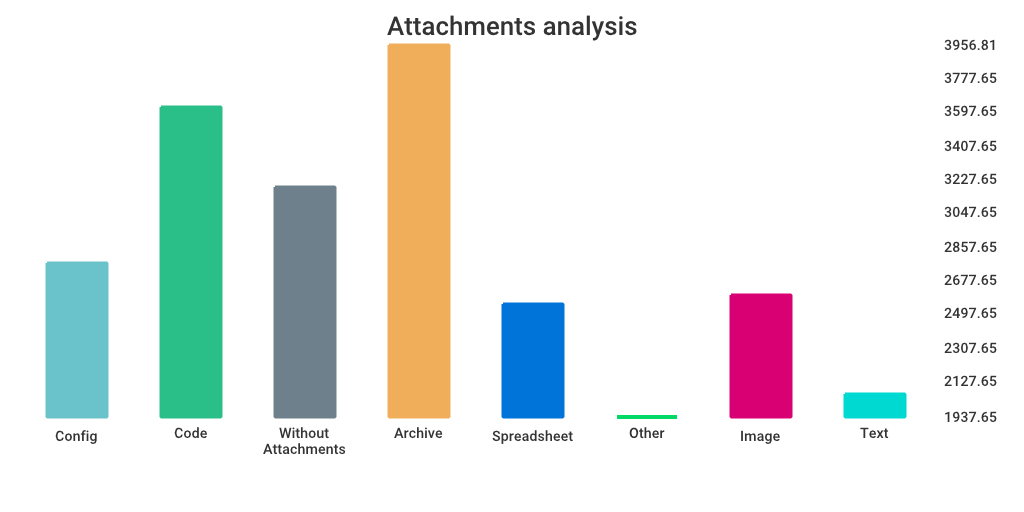
\includegraphics[scale=0.23]{images/attachments.png}
  \end{center}
  \caption{\label{attachments}Attachments analysis.}
\end{figure}

Attachments are, as mentioned previously, files attached to software tickets that can take any form - from code 
snippets written in Java to tar archives. We have analyzed all tickets that were both of high priority tickets and
were marked as Closed by the time we collected the data. Then we split all these tickets into two main categories: 
with attachments and without attachments. Furthermore, the tickets that were marked as having attachments were split 
into the categories specified in Section \ref{characterising}. In total, we looked at 201,786 tickets, among which 
98,311 had attachments and 103,475 without any attachments.

Using the plot package in our Go tool, we automatically generated the bar chart shown in Figure \ref{attachments}. 
As it can be seen, various types of attachments can produce completely different \emph{times-to-close}. For 
tickets with archive we can see the longest time-to-close mean while tickets having text attachments are at 
the other end of the spectrum. The smallest mean is for other attachments, which is represented by any file 
that does not have an extension specified in one of the other categories. 

We assume that image attachments are screenshots attached to the ticket in order to help developers see and 
subsequently reproduce the bug. Thus, we can clearly see that the difference between the means of time-to-close 
for tickets without attachments and tickets with screenshots is significantly in favor of the latter. This can 
indicate that developers indeed find screenshots helpful in solving the ticket faster.

Another insightful result is the fact that having text, config and spreadsheet attachments significantly 
reduces the time-to-close for the ticket. This can imply that developers find value in various steps to reproduce, 
config values used by users when the bug encountered or data in a spreadsheet format (e.g. csv) that can be 
found in such files and helps them lower the time-to-close for the ticket.

On the other hand, having no attachments does not necessarily mean that the ticket will get closed after 
a longer period of time. As it can be seen in the figure, the mean time-to-close value for tickets without 
attachments is somewhat neutral in the entire data set.

However, we need to take into consideration tickets that have code attachments which are a \emph{thread to validity}. 
When a snippet of code is attached, it might result in more complex tickets due to developers spending more time on 
understanding what is going on and reasoning about the attached code. Also, engineers might need to run or test 
the code attached which can again increase the Time-To-Close.

A Welch T Test was computed to test the difference between tickets with attachments and those 
without attachments. The analysis revealed significant difference with $p > 0.01$ with an
average of $1380.551$ hours for tickets with attachments and an average of $3180.882$ hours
for tickets without attachments. 

Thus, our analysis shows that having attachments in most formats, ranging from markdown files to PNG screenshots 
and snippets of code, can help developers solve the tickets faster. We believe that the solution of making attachments
provide the most value to the software project would be if issue tracking systems would make explicit to the reporters 
that uploading a screenshot or a code snippet can help reduce the time-to-close for the ticket.

\subsection{Steps to Reproduce}

\begin{figure}[ht]
  \begin{center}
    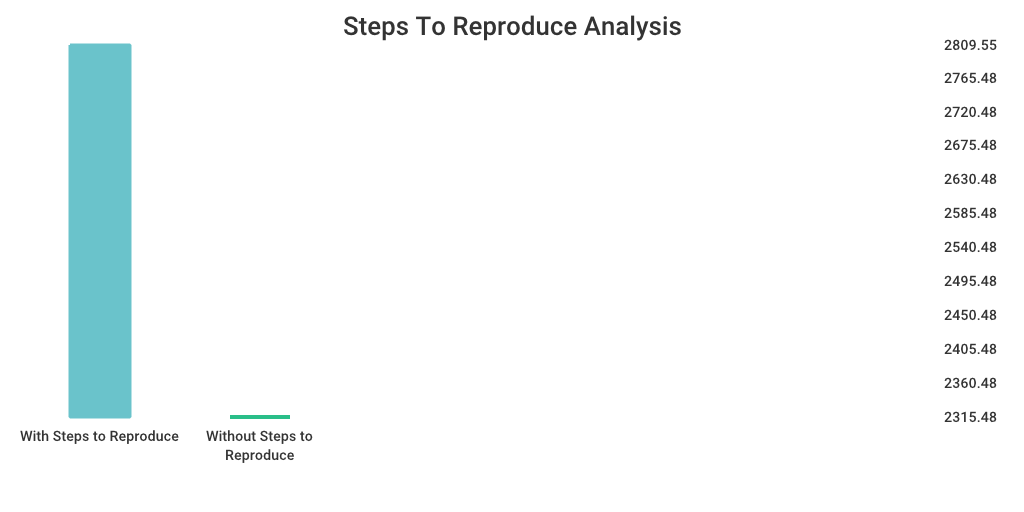
\includegraphics[scale=0.23]{images/steps_to_reproduce.png}
  \end{center}
  \caption{\label{steps}Steps to reproduce analysis.}
\end{figure}

Steps to reproduce are a means of specifying to the developers what actions they need to undergo in order 
to reproduce a certain bug. They can take various forms, but as Jira uses a wiki style markdown format for 
their description and comments fields, they can be inserted as a bullet point list which can be easily 
extracted with a regular expression.

Figure \ref{steps} shows the bar chart representing all closed, high priority tickets with or without steps 
to reproduce in either the description field or in any of the comments. We looked in total at 201,786 tickets 
among which 31,732 tickets had steps to reproduce and 170,054 did not have.

As it can be shown in the figure, having steps to reproduce can significantly reduce the time-to-close 
for the ticket. Even though the data collected does not have such many tickets with steps to reproduce 
(39,988 compared to the total number of 238,286 closed tickets), it is still a valuable finding which shows 
that steps to reproduce are indeed a quality factor for software tickets. 

What we can infer from this result is that steps to reproduce reduce the communication friction between 
the reporters and the developers - in the case of a bug which is harder to reproduce (e.g. maybe the 
bug occurs only on Linux and the developer is running MacOS, but the reporter did not specify his/her 
operating system in the ticket), the developer might need to contact the reported either directly or 
through commenting on the issue. What this implies is waiting time until the reporter comes back on the 
issue tracking system or sees the notification that he/she received a new message, which subsequently makes 
the ticket remain open for a longer period of time. 

A Welch T Test was computed to test the difference between tickets with steps to reproduce 
and those without steps to reproduce. The analysis revealed significant difference with 
$p < 0.01$ with an average of $1596.714$ for tickets with steps to reproduce and an average of 
$2609.142$ for tickets without steps to reproduce.

Thus, the answer to our research question is that the presence of steps to reproduce in tickets 
has a positive influence on the time-to-close. One solution that we propose for maximizing their benefit 
is that issue tracking systems should include hints on the ticket creation form specifying that 
steps to reproduce should be included as developers would be able to fix the bug faster. Moreover, 
issue tracking systems could also automatically add a new system field (like summary or description) 
for any project created and the project maintainers or administrators could make them mandatory for 
when a ticket is created by reporters.

\subsection{Stack Traces}

\begin{figure}[ht]
  \begin{center}
    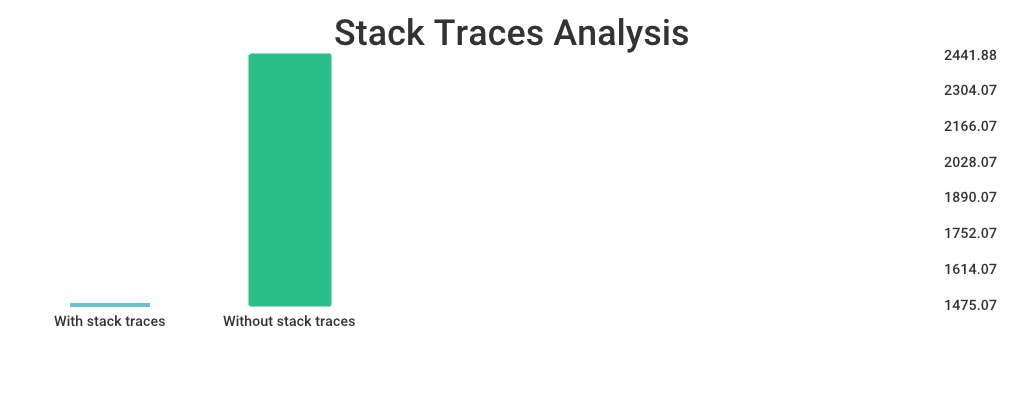
\includegraphics[scale=0.23]{images/stack_traces.png}
  \end{center}
  \caption{\label{stack_traces}Stack traces analysis.}
\end{figure}

Stack traces are active stack frames at a certain point in time while the program is executing. 
Many programming languages provide stack traces through their standard libraries, but the most 
popular proponents are Java and C\#. As Java is the main programming language used throughout 
the Apache Software Foundation projects (231 projects \cite{apache_projects}), many of the projects 
we collected (22) are also written in Java, thus we had a considerable chunk of data to analyze.

For this analysis, we only looked at tickets of high priority, closed and the project they correspond 
is written in Java. In total, we investigated looked at We then ran a complex regular expression derived from the works of Bettenburg et. al 
\cite{bettenburg2012using} and Moreno et. al \cite{moreno2014use} and collected all the tickets that have 
stack traces. In the end, we got a total number of 256 tickets that had at least an exception stack trace 
attached in either summary, description or any of the comments.

As shown in Figure \ref{stack_traces}, we can see that the presence of exception stack traces can 
reduce the time-to-close of a ticket in orders of magnitude. This could imply that stack traces help 
developers working on the project localise the code that is running exceptions 

We computed a Welch T Test to test the difference between tickets with stack traces and tickets that 
do not have stack traces. The analysis revealed significant difference with $p < 0.01$ with an
average of $1475.074$ for tickets with stack traces and an average of $2441.877$
for tickets without them.

\subsection{Comments}

\begin{figure}[ht]
  \begin{center}
    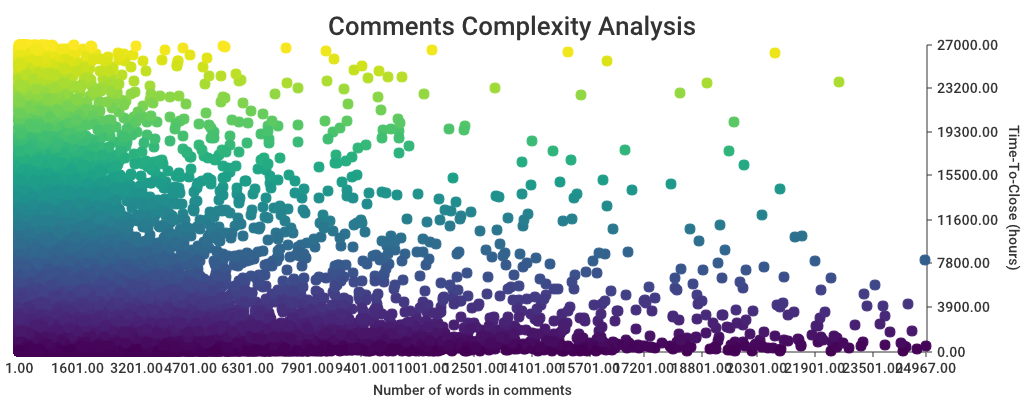
\includegraphics[scale=0.23]{images/comment_complexity.png}
  \end{center}
  \caption{\label{comments}Comments complexity analysis.}
\end{figure}

The comment field is comprised of a textual body, a corresponding author, its time of creation and any updates 
that were performed on it throughout its lifecycle. They provide a space for developers and end users to discuss 
anything related to the ticket they belong to. Any popular issue tracking system, such as Jira, does not enforce 
any limit on any component of a comment, thus the number of words for a single comment can range from only 5 
to well over 1,000. 

We concatenated all comments into a single large string in order to be analysed for total number of words. This step 
was performed at the end of each ticket's lifecycle. We ran our comments analysis on 201,786 tickets among which 
113,344 had comments and 88,442 did not have any comments. 

In Figure \ref{comments} we present the correlations between the total number of words in comments per ticket and 
the corresponding Time-To-Close for that ticket. We can observe in the scatter plot that most tickets tend to 
have up to around 3,200 words in total. However, there are tickets that have a total number of words as high as 
around 25,000. 

From the figure we cannot clearly deduce whether increased number of words in comments influence 
the Time-To-Close positively or negatively. However, a correlational analysis releaved a weak 
positive relationship with $r = 0.271$ and $p < 0.01$. This implies a statistically significant finding - 
as the number of comments increases, the quality of the ticket decreases. 

Even though this might be surprising at first, we need to analyse the possible context where such large 
number of words in comments occur. What if the bug was so hard to reproduce that the developers needed to 
ask more than one user how they experienced the issue in the tool? Another case might be that even though 
the comments start by discussing fixing or implementing a feature, the developers and end users might 
engage in new conversations about the product in general or other features that they might want to see 
implemented. Also, what if comments are a means of communication for developers in the team? There are studies, 
such as the one conducted by Lotufo et. al \cite{lotufo2015modelling}, that show the importance of comments 
in software tickets in relation to communication activities surrounding the project. Another possible explanation 
for having increased number of comments increase the Time-To-Close value and, thus, decrease quality, is that 
having many comments or very verbose comment can lead to more difficult information extraction. On the other 
hand, if there would be a light discussion, the developers would be able to quickly analyse all the comments 
and collect whatever is necessary to resolve the ticket.

One possible solution that we propose to this correlation is to have the ability to limit the number of 
comments per ticket. As to our knowledge, one cannot do this in neither Jira nor Bugzilla. However, if it were 
possible, we believe that this might help developers find the information they need quicker. But what happens 
if the treshold is reached and there is still a need for clarifying certain aspects? We believe that having 
a button redirecting anyone still interesting in commenting on the ticket to a messaging tool, such as 
Slack, would be beneficial for the project overall. Thus, if they were redirected to let's say Slack, a small 
tool could automatically be run that creates a new channel specifically for that ticket with the name set 
to the unique ticket key (e.g. LUCENE-2901). We believe that such a solution could aid both developers in 
completing tasks quicker but also end users for feeling more involved and valuable to the project.

\subsection{Summary and Description}

\begin{figure}[ht]
  \begin{center}
    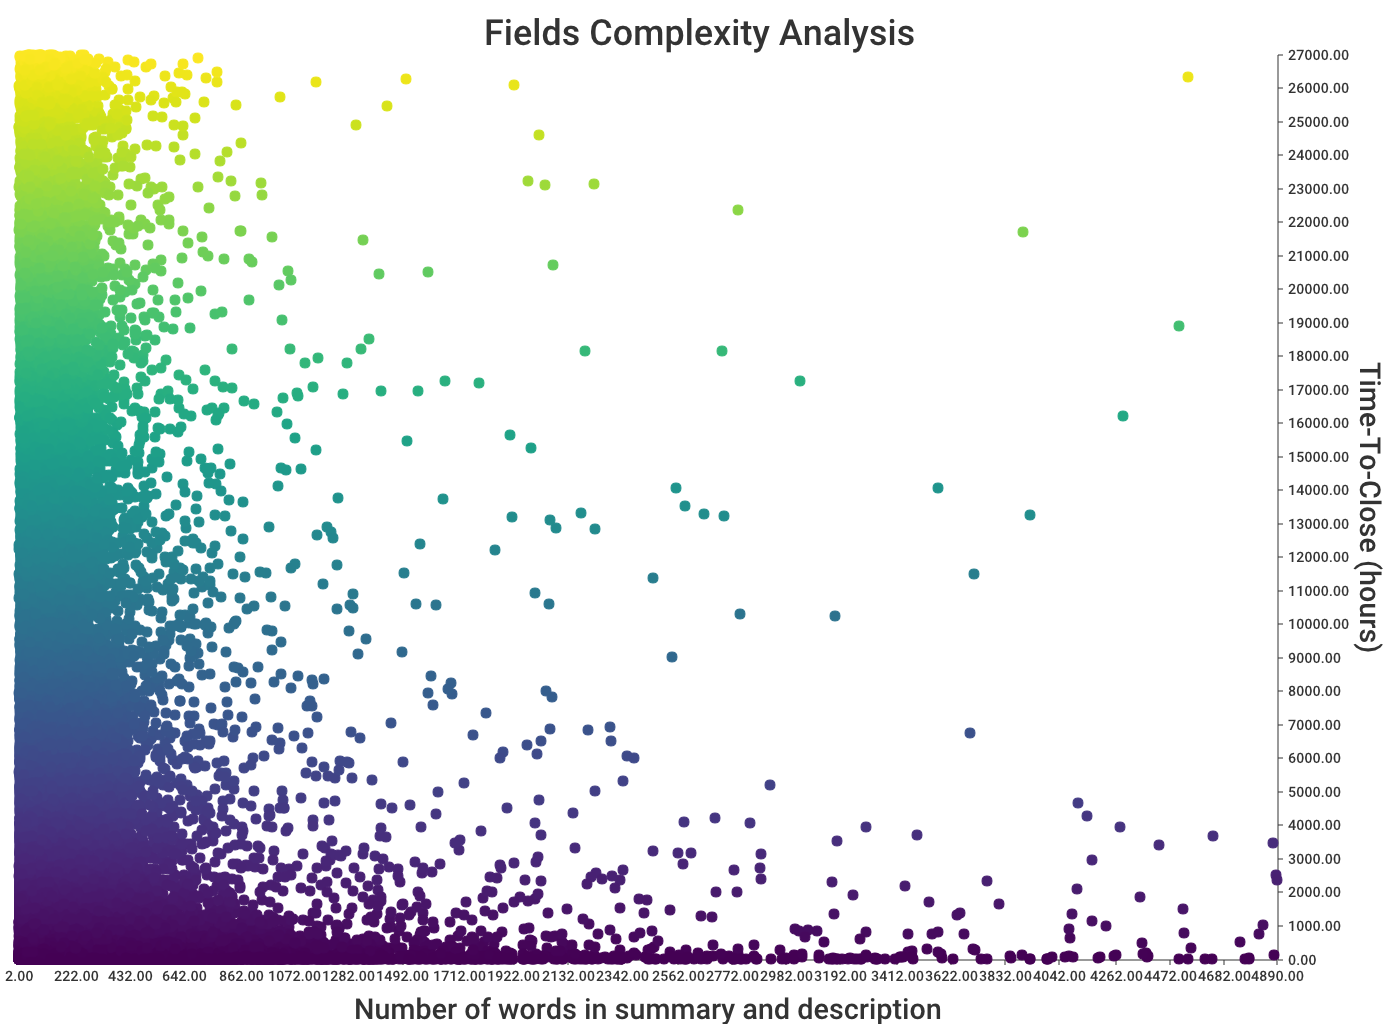
\includegraphics[scale=0.23]{images/fields_complexity.png}
  \end{center}
  \caption{\label{fields}Time-To-Close versus summary and description word count.}
\end{figure}

Summary and description are the two most important and most frequently completed fields in a ticket on any
issue tracking system. Even though summary is required on any issue tracking system, description might 
be omitted if the reporter does not feel the need of adding any extra detail other than what is in the summary. 
However, as bug reports are usually complex, there is a very small percentage of descriptions not filled in 
by the reporters. They do not typically have any word limits, thus the reporter can add as much information as 
they see fit.

Figure \ref{fields} shows the scatter plot for the sum of numbers of words in summary and description, as well 
as the Time-To-Close for the ticket. We have analysed a total number of 238,286 tickets, as they all have both 
summaries and descriptions. We concatenated the summary and description for every ticket at the end of the ticket 
lifecycle.

The Figure shows a very similar correlation to the one for comments complexity. A correlational analysis revealed 
a weak positive relationship with $r = 0.178$ and $p < 0.01$. This implies both that our results are statistically 
significant and also that as number of words in summary and description increase, the Time-To-Close increases, thus 
the quality of the ticket decreases.

This is not a surprise - as previously mentioned, summary and description are the core components of any ticket. 
As summary is described by Jira, it should represent a short textual description of the bug or the feature request. However,
we have identified tickets having summaries with even more than 200 words. This is not optimal and might obfuscate
the essential reason of filing that ticket from triagers and developers working on the project. One of the findings 
Zimmermann et. al \cite{zimmermann2010makes} present in their study is that a good, succint summary can significantly 
reduce the effort invested by the developers. 

Description, on the other hand, even though it is made to be a more detailed summary of the report, it should still be
in some reasonable parameters. During our analysis process, we identified more than 50 tickets having descriptions 
with more than 4,000 words. Even though they included various types of information, including steps to reprodce, 
we believe that the reason why Jira and the other popular issue tracking systems created so many fields for bug reports 
is that the information that could all be put in description should be split across these fields: 
\begin{itemize}
  \item if there are stack traces or steps to reproduce, as we mentioned above, there should be specific fields 
  created exclusively for them; 
  \item if the end user is an experienced one and has reported numerous bugs or feature requests for the project, 
  they might also be able to provide an estimate for the difficulty of the task; however, that should be stored in the 
  Jira system field called \"Story Points\";
  \item the user might also want to provide excerpts of code or previous discussions with other end users/developers; 
  however, they should not upload it inside the description field, but rather create a text attachment (e.g. markdown
  document) and attach it separately so that they keep the description clean and easy to follow.
\end{itemize}

A solution for this issue could be the freedom of easily selecting the total number of words allowed for summary and 
description. Even though this is possible with Jira, the process of configuring it is not trivial, thus many 
administrators do not perform this step. An even better approach would be to have a tool automatically generating 
word limits based on, for example, the experience of the reporter - if he/she has significant knowledge regarding 
the project, they should be allowed to include lengthier summaries or descriptions mainly because they are more inclined 
to know that without a very good reason, following this approach is not the most optimal way. 

Another simple and straightforward solution can be the simple addition of hints below or above the text boxes for summary 
and description where administrators can write succint messages adivising reporters to not write verbose paragraphs 
unless they really have a very good reason to do so.

\subsection{Grammar Correctness}

\begin{figure}[ht]
  \begin{center}
    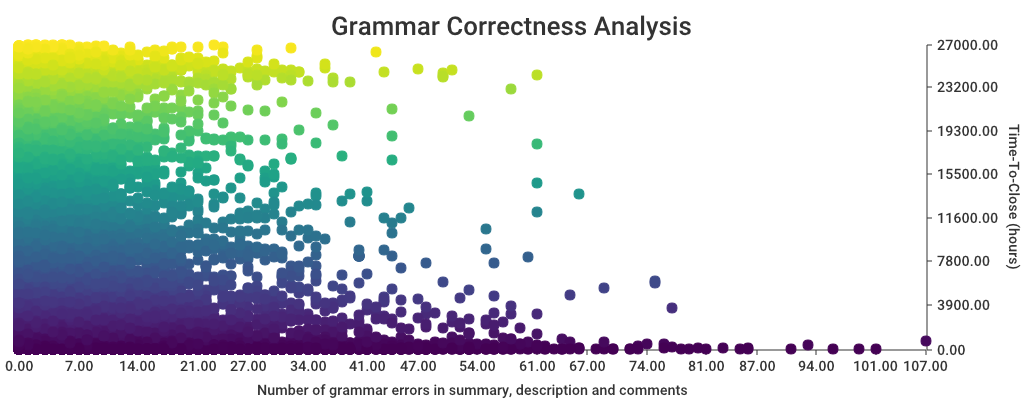
\includegraphics[scale=0.23]{images/grammar_correctness.png}
  \end{center}
  \caption{\label{grammar}Grammar correctness score analysis.}
\end{figure}

Through calling Microsoft Azure's Bing Spell Check API, one of the best grammar analysis APIs in the industry, we 
managed to calculate the total number of grammar errors in summary, description and comments for a total number 
of 133,689 tickets. As shown in a number of studies, the number of spelling errors can influence the quality of a ticket. 
However, in the work conducted by Schugerl et. al \cite{schugerl2008mining}, the authors found that spelling errors 
can be found in both high and low quality tickets, thus should not be considered as a reliable factor for determining
the Time-To-Close for a ticket. In the rest of this section we will demonstrate the contrary - tickets with more 
grammar errors (spelling errors are just a subset of the types of errors we are investigating) imply lower quality
tickets. 

This analysis type is called grammar correctness rather than spelling scores because the range of errors returned 
by Bing Spell Check API are of many types, some of which are:
\begin{itemize}
  \item spelling errors; however, they go much further than a simple character mistyped - for example,
  if one would type Micrsft, it would automatically flag it as a grammar error because it also takes into account a large 
  database of words not in standard dictionaries, but also popular words in the tech world (e.g. company names) or 
  jargon language (e.g. dab dance);
  \item contextual errors - e.g. I ate a book today; even though this is not a misspell, the API will return \emph{book} as 
  a grammar error due to the fact that it is used in the wrong context;
  \item it can detect the wrong usage of a verb tense in a specific context;
  \item it can flag wrong conjugations of verbs;
\end{itemize}

After concatenating the strings for all comments, summary and description, we ran our analysis and then plotted the 
data which is depicted in Figure \ref{grammar}. A correlational analysis revealed a weak positive
relationship with $r = 0.134$ and $p < 0.01$. Thus, our results are statistically significant, implying that 
having more grammar errors in a ticket will increase the Time-To-Close for a ticket and, thus, decrease the quality. 

This is expectable as having a text difficult to grasp and understand makes it harder to reason about what needs 
to be done in order to fix a ticket. As it can be seen in the graph, most tickets are concentrated in the range of 
0 to 40 grammar errors per ticket. Having 40 grammar errors in a ticket is quite a large number, considering the fact 
that many tickets don't have comments at all and summary and description are not large in general. 

However, we can not automatically change this through automation like the solutions we presented in the previous 
analysis types. We cannot call, for example, the Bing Spell Check API every couple of seconds on the text the user 
is inputting in the ticket as the costs would become unbearable very soon. Thus, what can be done to fix this? It is, 
after all, in the human nature to make mistakes, and typing is no exception. If we, for example, have some hint or a rule
in the code of conduct for the project stating that everything should be 100\% gramatically correct, many reporters not 
having English as their primary language would feel unwelcomed and they might not get involved in the project anymore. 

The solution we are proposing implies a local, lightweight spell checker that is run automatically as the user types. 
This tool would not make any external calls, so there would be no costs and the load on the server would also be lower. 
There are already local applications that can be used for performing such real-time analysis on the text, one of them 
being LibreOffice's built-in spell checker.

\subsection{Sentiment Scores}

\begin{figure}[ht]
  \begin{center}
    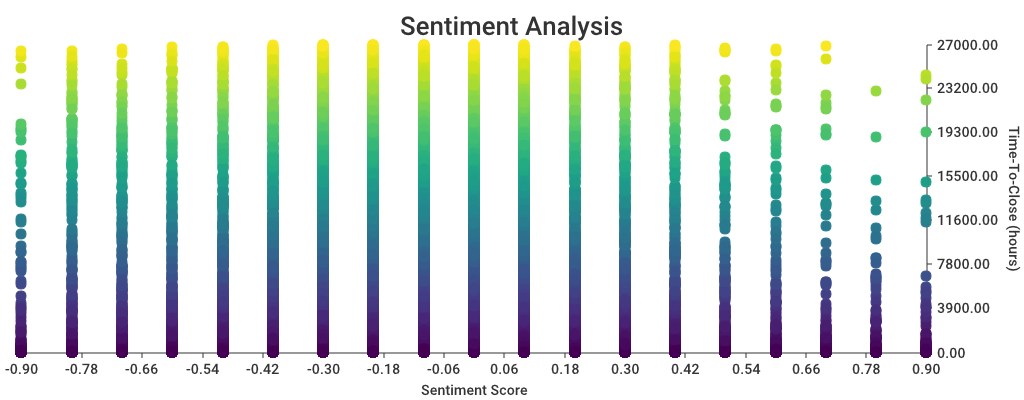
\includegraphics[scale=0.23]{images/sentiment_analysis.png}
  \end{center}
  \caption{\label{sentiment}Sentiment score analysis.}
\end{figure}

Sentiment analysis is a technique of employing Machine Learning algorithms in order to infer a sentiment 
score from textual information. These algorithms need to be trained on very large data sets in order to 
produce valuable results. Moreover, we would have also needed an already annotated data set, which means 
a number of strings where we compute the score by hand given a mathematical formula we define. Even though 
there are open source libraries that can help creating and employing the algorithms, such as TensorFlow, 
we would still have needed tickets where we defined what do we mean by positive/negative tickets, as well as
manually computing the scores for a large range of them. Therefore, we ended using a third party API - Google 
Cloud Platform Natural Language Processing, considered the best such service at the moment. This API returns 
a score between -1 (most negative) and +1 (most positive) for any text encoded in the HTTP request.

After we concatenated summaries, descriptions and all the comments for every ticket, we started sending our 
requests to Google and we plotted the data shown in Figure \ref{sentiment}. A correlational analysis revealed a 
weak negative relationship with $r = -0.114$, $p < 0.01$. Therefore, we obtained statistically significant 
results implying that as the sentiment decreases (i.e. becomes more negative), the Time-To-Close increases, thus 
decreasing the quality of a ticket.

We can see in the Figure that neutral scores (i.e. between -0.42 and 0.42) show rather neutral results, which 
was expectable: this most probably implies that the discussions and descriptions for these tickets revolved 
completely around the ticket and nothing else. 

However, as the sentiment decreases, we can clearly observe that the sentiment scores increase significantly. 
This might signify that once the discussion becomes \"heated\", the developers might lose interest in solving 
the task anymore. Also, rude language might be a driver for increased Times-To-Close because when developers are 
answering questions from the reporters (or vice versa), the other person might become rude or unpolite, which can 
make them feel unwelcomed and start to lose interest in helping the project anymore. 

On the other side of the spectrum, having a more positive score leads to higher quality in tickets. Calefato et. al 
\cite{calefato2015mining} conducted a study where they show that a positive sentiment has the biggest impact on 
the quality of an answer on Stack Overflow, one of the most popular websites related to programming in general. This 
implies that when developers and triagers treat their reporters respectfully and offer support whenever possible, 
the users will feel more welcomed and willing to help report other bugs in the future as well. We also have scores of 
over 0.9, meaning that the actors participating in the discussion (or the reported summary/description) might compliment 
each other for doing a great job.

We strongly believe that having a positive sentiment score for tickets is valuable for absolutely everyone: the company
behind the projects sees increased overall performance and productivity, developers feel better working in the team or
on that specific tool and reporters will be more willing to contribute in the future with other tickets.

A solution for pushing towards this ideal scenario would be expensive for the company, but the most efficient - have a 
sentiment analysis tool running in the background as the user is typing in any text box. If they reach a certain low 
treshold and it is believed that they are becoming rude or unpolite, there could be a warning/pop-up on the screen advising 
them to not do that as it wouldn't help any party, but rather try to be polite, engaging and friendly. One other solution
is a much more cost-effective one, but less efficient - the issue tracking system administrators could include a section 
in the code of conduct for the project stating that promoting a positive environment will help everyone. This way, people 
revolving around the project might be more inclined to be friendly.

\section{Future Work}\label{future_work}

The first extension to the Go tool we created would be to add support for Bugzilla. We already achieved this 
when we were first prototyping the application, but we decided to proceed exclusively with Jira mainly because 
the APIs proved to be more reliable and also versatile in terms of what data you could collect. Another 
reason was that we were time retricted, thus we wanted to have first a well tested and stable solution for Jira and 
only after add support for other issue tracking systems. However, we already prepared for other potential systems by 
adding interfaces for tickets and REST clients, making Bugzilla, Manuscript, YouTrack or any 
other issue tracking system straightforward to add to the application.

One other improvement to the application could be adding more robust support for statistical analysis. At the moment, 
our tool uses our own custom types and functions for generating Welch T Test and Spearman R Test results, and even if 
it produces the expected \emph{p} and \emph{r coefficient} values, end users of the application might want to 
analyse even more possible correlations. As the Go community lacks native libraries to perform statistical tests, 
the users of our tool might miss the simplicity of running such tests in R. A solution can be to integrate the 
Roger library \cite{r_stats} inside the stats package, which basically allows any Go application to communicate with 
R via TCP. 

There is also room for future work in terms of the data collected. Even though the database we collected 
is large, there is never enough tickets to analyse. Thus, the store command of the tool could be run against 
other Jira instances apart from Apache's and collect tickets from other projects, thus improving the diversity 
and the total number of tickets to be analysed. As we did not have access to any cluster or virtual machines in 
the cloud, we ran all our analyses on local machines (laptops) and it could still take well over two hours to complete 
with over 10 GB of RAM and 70\% CPU in usage.

Furthermore, the project could greatly benefit from having access to closed source repositories in addition to the 
open source ones. Most closed source projects have much more structured planning, tracking and management activities - as 
Crowston et. al \cite{crowston2012free} present in their study, open source projects lack organized coordination which,
in the context of our study, means that people do not invest much effort into properly creating tickets in issue tracking 
systems, triaging efficiently, planning the work and tracking it. On the other hand, closed source projects follow 
more strict guidelines: standard working hours (would make tracking and linking the source code changes to tickets easier), 
adding story points (i.e. adding estimated difficulty or time to complete) and properly planning tickets before work 
starts on the task, tickets properly distributed to developers based on availability and expertise etc. These benefits 
of closed source projects would prove helpful for our analysis.

Another aspect that could be improved is having access to funds in order to buy Google Cloud Platform credits. This 
would be required to use the Natural Language Processing APIs on large amounts of data. We used the credits provided 
in the free trial but quickly ran out completely after only 160,000 tickets. Also, credits on Microsoft Azure would 
prove useful as their Spell Check API is the most efficient at the moment.

A major future work candidate is availability of a technique to calculate the difficulty of a ticket based on the information
inside it. Unfortunately, at the moment, the research community has not come up with such an approach. 
Vijayakumar et. al \cite{vijayakumar2014much} proposed a method of predicting how much effort is required for fixing 
a bug, but after running it on our data, it did not prove successful. After such a technique becomes available, we could 
incorporate it inside our tool and group the tickets compared in all analysis types based on their difficulty in order to 
have better results.

We wish that our final deliverable would be either a \emph{goodness} metric, describing the quality of a ticket based 
on the information inside, or a recommender tool that could automatically create high quality tickets. This requires 
intensive work over a longer period of time, but we believe that with the findings presented in this study together 
with other state-of-the-art research in the field, it is possible to implement it.

\section{Conclusions}\label{conclusions}

Software tickets are a vital part of every software project's lifecycle. Even though there might be other means
of planning, managing and tracking work for a software team, issue tracking systems are deployed in virtually any company
that provides a computer application or service.

Deriving a quality score only from textual information and other non-structured data such as images is not trivial. 
However, in this study we managed to create an application that can automatically fetch and store tickets from any 
Jira instance, analyse them and compute statistical tests and graphs.

We manager to answer all seven research questions and find factors that can posittively or 
negatively affect the quality of a ticket. All of our results are statistically significant and we can summarise 
them as follows:
\begin{itemize}
  \item the presence of steps to reproduce increases the quality of a ticket;
  \item the presence of stack traces increases the quality of a ticket;
  \item the presence of attachments increases the quality of a ticket - more specifically tickets with screenshots, 
  config files or text files have lower times-to-complete than tickets without attachments;
  \item higher numbers of grammar errors impply lower quality scores for a ticket;
  \item higher sentiment scores imply higher quality scores for a ticket;
  \item higher numbers of words in comments imply lower quality scores for a ticket;
  \item higher number of words in description and summary imply lower quality scores for a ticket.
\end{itemize}

We intend to continue work on the project and implement the points we have listed in Section \ref{future_work}. We believe
that by open sourcing the application and making the data publicly available, we can provide a valuable starting point 
for other studies investigating this particular field of software engineering.

\vskip8pt \noindent
{\bf Acknowledgments.}
I would first like to thank Dr. Storer for the amazing work he has put in helping me go through with finishing 
this project. I would definitely not have been able to achieve what we've achieved with any other supervisor, so 
thank you, Tim, for all the support, kindness and advice you have given me throughout this academic year. I would 
also like to thank you for being the lecturer who has taught me the most throughout all my years at the university
and whose advice and ideas I have applied at all my work places and my personal projects.

The next huge thank you would have to go to my parents, the most amazing family in the world! Without them I would 
not be here and I wouldn't have had anything of what I have now, both personally and professionally. 
I will always treasure the unconditional support you have always offered me! Thank you for being my parents, Mom and Dad!

And last but not least, I want to thank my partner in \"crime\" and in life, Corina! Without her, I would not be who I 
am today. You have been with me through thick and thin, in both bad moments (such as the endless nights working 
on ticket statistics) and best moments in my life! Thank you for everything! I will always love you!

\bibliographystyle{abbrv}
\bibliography{paper}

\end{document}